\chapter{DUNE Physics}
\label{ch:exec-phys}


%%%%%%%%%%%%%%%%%%%%%%%%%%%%%%%%%%%%%%%%%%%%%%%%%%%%%%%%%%%
%\section{}
%\label{sec:exec-phys-1}
%
%%%%%%%%%%%%%%%%%%%%%%%%%%%%%%%%
%\subsection{}
%\label{sec:exec-phys-2}

The aim of this chapter is to summarize the 
DUNE scientific program.  
%This summary includes an 
%illustrate the present understanding of the capability to 
%realize the scientific opportunities for which DUNE has been designed.
%
%
%In this chapter,
Presented here in summary form are   
(1) the scientific goals and opportunities, 
(2) the key features of the experiment 
design that enable this program, 
(3) the methodologies we have 
employed to evaluate the capabilities of DUNE to realize 
the science, 
(4) the corresponding results for selected program elements, 
and (5) the demands placed on the experiment design and 
performance.

%%%%%%%%%%%%%%%%%%%%%%%%%%%%%%%%%%%%%%%%%%%%%%%%%%%%%%%%%%%%%%                                   
\section{Goals of the DUNE Science Program}
\label{sec:exec-phys-key-goals}

The LBNF/DUNE strategy has been developed to meet the
requirements set by the US Particle Physics Project Prioritization Panel
(P5) in 2014. It also takes into account the recommendations
of the European Strategy for Particle Physics (ESPP) adopted
by the CERN Council in 2013, which classified the \dword{lbl}
neutrino program as one of the four scientific objectives that
require international infrastructure.

As a benchmark, the P5 report~\cite{p5report2014} set the goal of
reaching a sensitivity to \dword{cpv} of better than three
standard deviations (\num{3}$\sigma$) over more than $75\%$
of the range of possible values of the unknown
\dshort{cp}-violating phase \deltacp.
Based partly on this goal, it stated that ``the
minimum requirements to proceed are the identified capability
to reach an exposure of \num{120}~\ktMWyr{} by the 2035 time
frame, the far detector situated underground with cavern space
for expansion to at least \fdfiducialmass \lar fiducial volume,
and \SI{1.2}{MW} beam power upgradeable to multi-megawatt power.
The experiment should have the demonstrated capability to
search for \dwords{snb} and for proton decay, providing a
significant improvement in discovery sensitivity over current
searches for the proton lifetime.''
These requirements are discussed below and in the sections
that follow.

To summarize, the DUNE experiment will combine the world's most
intense neutrino beam, a deep underground site, and massive \lar
detectors to enable a broad science program addressing some of
the most fundamental questions in particle physics.
This program is articulated in brief form below.

The primary science goals of DUNE are to:
\begin{itemize}

\item Carry out a comprehensive program of neutrino oscillation measurements using
      \numu and \anumu beams from \fnal. This program includes measurements of
      the \dword{cp} phase, determination of the neutrino mass ordering
      (the sign of \dm{31}$ \equiv m_3^2-m_1^2$), measurement of the mixing
      angle $\theta_{23}$ and the determination of the octant in which this
      angle lies, and sensitive tests of the three-neutrino paradigm.
      Paramount among these is the search for \dword{cpv} in neutrino oscillations, potentially offering 
      insight into the origin of the matter-antimatter asymmetry,
      one of the fundamental questions in particle physics and cosmology.

\item Search for proton decay in several important decay modes.
      The observation of proton decay would represent a ground-breaking discovery
      in physics, satisfying a key requirement of grand unification of the forces.

\item Detect and measure the $\nu_\text{e}$ flux from a core-collapse
      supernova within our galaxy, should one occur during the lifetime
      of the DUNE experiment. Such a measurement would provide a wealth
      of unique information about the early stages of core-collapse, and
      could even signal the birth of a black hole.

\end{itemize}

The intense neutrino beam from LBNF, the massive DUNE \lartpc
far detector, and the high-resolution DUNE near detector will also
provide a rich ancillary science program, beyond the primary goals
of the experiment. The ancillary science program includes:
\begin{itemize}

\item Other accelerator-based neutrino flavor transition measurements with
      sensitivity to beyond the standard model (BSM) physics, such as non-standard
      interactions (NSIs), Lorentz invariance violation, \dword{cpt} violation,
      sterile neutrinos, large extra dimensions, heavy neutral leptons,
      and tests with measurements of tau neutrino appearance;

     \item Measurements of neutrino oscillation phenomena using atmospheric neutrinos;


     \item Searches for dark matter utilizing a variety of
           signatures in both
           near and far detectors, as well as  
           non-accelerator searches for BSM physics 
           such as neutron-antineutron oscillation.

     \item A rich neutrino interaction physics program utilizing the DUNE near detector,
           including a wide-range of measurements of neutrino cross sections and studies of
           nuclear effects; and

\end{itemize}

Further advancements in the \lartpc %far detector 
technology during the course of the far detector construction
may enhance DUNE's capability to observe very low-energy
phenomena such as solar neutrinos or even the diffuse
supernova neutrino flux.

%%%%%%%%%%%%%%%%%%%%%%%%%%%%%%%%%%%%%%%%%%%%%%%%%%%%%%%%%%%%%%                                   
\section{Enabling LBNF/DUNE Operating Principles}
\label{sec:exec-phys-operatingprinciples}

World-wide scientific and technical planning for the
ambitious next-generation deep underground long-baseline
neutrino oscillation experiment that LBNF/DUNE now represents
has been under way for more than a decade.  Much
development preceded the formation of the DUNE science
collaboration in 2015 (see, for example,
Refs.~\cite{Adams:2013qkq} and \cite{LAGUNA-LBNO-deliv}).

Extensive study and discussion within the community
have led to the principal elements of the LBNF/DUNE
configuration:
\begin{itemize}
  \item {\bf\boldmath High-intensity conventional wide-band
  $\nu_\mu$ beam}\\
	The current generation of long-baseline neutrino experiments
	have benefited from narrow-band beam characteristics 
	associated with off-axis detector deployment. The principal 
	advantage is a low background rate in both \nue appearance 
	and \numu disappearance channels from misidentified neutral 
	current interactions of high energy neutrinos.  
	However, this advantage comes at a cost of flux and 
	spectral information relative to an on-axis detector 
    configuration~\cite{Adams:2013qkq,Agarwalla:2014tca}.
    The DUNE concept
    builds on the notion that a highly-performant detector
    technology with excellent neutrino energy reconstruction
    and background rejection capabilities can
    optimize sensitivity and cost with an on-axis exposure to
    an intense conventional (horn-focused) beam.

  \item {\bf Far detector site selection for long baseline}\\
    The 1300-km baseline offered by locating the DUNE far detector
    at the Sanford Underground Research Facility in Lead, 
    South Dakota is well-optimized for the neutrino oscillation 
    physics goals of the program~\cite{Bass:2013vcg}.

  \item {\bf Deep underground location for far detector modules}\\
    Early studies (see, {\sl e.g.}, Ref.~\cite{homestake:depth}) 
    demonstrated that to realize the non-accelerator based elements
    of the DUNE science program, a deep underground far detector
    location is required.  These studies also indicate that the 
    4850 Level of Sanford Lab provides sufficient attenuation of 
    cosmic rays in the rock above, conclusions that have been 
    supported by more recent studies (see,
    {\sl e.g.}, Refs.~\cite{bib:docdb3384,bib:docdb1752}).

  \item {\bf \lartpc technology for far detector modules}\\
    Combining intrinsic scalability with high-performance event 
    imaging, calorimetry and particle identification capabilities, 
    the \dword{lartpc} concept was developed 
    for a broad-based underground science program matching well 
    that of DUNE.  This design choice integrates well with the
    other elements and provides valuable complementarity to other 
    existing and planned detectors pursuing many
    of the same goals.  As an example of this complementarity,
    the sensitivity of DUNE to the \nue component of supernova 
    neutrino flux, prevalent in the neutronization phase of the 
    explosion, provides distinct information relative to that 
    provided by water or organic scintillator-based detectors in 
    which \anue interactions dominate.  It is also notable that 
    the value of excellent neutrino energy reconstruction capability
    is especially important for the long-baseline program with a 
    wide-band neutrino beam.
\end{itemize}

The scientific basis for the above foundational experimental
design choices has been examined and validated through extensive
review, undertaken at all stages of DUNE concept development.
Recent experimental and theoretical developments have only
strengthened the scientific case for DUNE and its
basic configuration.  The technical underpinnings for
these choices have also been strengthened over time through a world-wide
program of R\&D and engineering development, as described in a suite
of LBNF/DUNE project documents including this \dword{tdr}, as
well as in sources describing independent experiments and development
activities.

%%%%%%%%%%%%%%%%%%%%%%%%%%%%%%%%%%%%%%%%%%%%%%%%%%%%%%%%%%%%%%                                   
\section{Summary of Assumptions and Methods Employed}
\label{sec:exec-phys-assm-meth}

Scientific capabilities are determined assuming DUNE
is configured according to the general parameters described above.
Further assumptions regarding the neutrino beam and detector 
systems, and their deployment, are stated here in
Sections~\ref{sec:exec-phys-assm-meth-beamdetector} and
\ref{sec:exec-phys-assm-meth-deployment}. 

Determination of experimental sensitivities relies on the
modeling of the underlying physics and background processes,
as well as the detector response, including calibration and
event reconstruction performance and the utilization of data
analysis techniques and tools.
A brief discussion of the strategies employed is given below
in Sec.~\ref{sec:exec-phys-assm-meth-simreco}. 

\subsection{Beam and Detector}
\label{sec:exec-phys-assm-meth-beamdetector}

Physics sensitivities are based on 
the optimized design of the 1.2~MW neutrino beam and
corresponding protons-on-target per year assumed to
be 1.1 $\times 10^{21}$ POT.  These numbers assume a combined
uptime and efficiency of the \fnal accelerator complex and the
LBNF beamline of 56\%.\footnote{This projection, from which one  
year of LBNF beam operations can be expressed as \SI{1.7e7}{seconds}, 
is based on extensive 
experience with intense neutrino beams at Fermilab, and in particular 
the NuMI beam line, which incorporates elements like those in the  
proposed LBNF beamline design and faces similar operating conditions.} 
%The beam design, simulation and associated
%uncertainties are described in
%Sec.~\ref{sec:physics-lbnosc-flux}.

For the neutrino oscillation physics program, it is assumed that
equal exposures (time-integrated beam power times fiducial mass) are obtained with both horn current polarities,
and therefore with the corresponding mix of primarily \numu
and \anumu data samples.
% (see Sec.~\ref{sec:physics-lbnosc-osc}).

It is assumed that the DUNE far detector will include some
combination of the different \nominalmodsize fiducial volume
implementations (single or dual-phase) of the \lartpc concept
for which technical designs have been developed.
%(see Sec.~\ref{sec:exec-scope}).                                                                
For much of the science program it is expected that the
capabilities of the two proposed far detector module 
implementations will be comparable.  As a result of the
current state of reconstruction and analysis software development
(see Sec.~\ref{sec:exec-phys-assm-meth-simreco}), the
physics sensitivity studies reported in this \dword{tdr} are based on
the single-phase \lartpc implementation,
documented in full in Volume~\volnumbersp{}, \voltitlesp{}.

It is also assumed that validation of the DUNE far detector 
designs will come from data and operational experience acquired 
with the large-scale ProtoDUNE detectors staged at CERN, 
including single-particle studies of data obtained 
in test-beam running.  

The near detector for DUNE has been under active development,
and a \dword{cdr} is in preparation.
Correspondingly, the descriptions utilized in this \dword{tdr}
are consistent with this level of development.  

\subsection{Deployment Scenario}
\label{sec:exec-phys-assm-meth-deployment}

Where presented as a function of calendar year,
sensitivities are calculated with the following
assumed deployment plan, which is based on a
technically limited schedule:
\begin{itemize}
    \item Start of beam run: Two \dword{fd} module %FD 
    volumes for total fiducial mass of 20 kt, 1.2 MW beam
    \item After one year: Add one \dword{fd} module  volume for total fiducial mass of 30 kt
    \item After three years: Add one \dword{fd} module  volume for total fiducial mass of \fdfiducialmass
    \item After six years: Upgrade to 2.4 MW beam
\end{itemize}


\subsection{Simulation, Reconstruction and Data Analysis Tools}
\label{sec:exec-phys-assm-meth-simreco}

The development of algorithms and software infrastructure needed
to carry out physics sensitivity studies has been an active 
effort within DUNE and the associated scientific community.  
Significant progress has been made: event reconstruction 
codes can be run on fully simulated neutrino interaction events 
in DUNE far detector modules; the DUNE computing infrastructure 
allows high-statistics production runs; and end-user interfaces 
are functioning.  Robust end-to-end analyses not 
possible a year ago have now been done and are being 
reported in this document.

For some aspects -- for example, beamline modeling
and GeV-scale neutrino interaction simulations --
well-developed and validated (with data) software packages have
been available throughout much of DUNE's design phase.
For others, corresponding tools did not exist and needed to be
either developed from scratch or adapted with substantial
modifications from other experimental programs.  Concurrent
with these development efforts, interim descriptions such
as parametric detector response modeling, necessarily crude
but based on reasonable extrapolation from experience and
dedicated studies, were employed to assess physics capabilities.
Even for the case of the better-developed tools -- again, neutrino 
interaction modeling is a good example -- significant incremental
improvements have been made as data from neutrino experiments
and other sources have become available and as theoretical
understandings have advanced.

As a result of the rapid pace of development as well as 
practical considerations including human 
resource availability, different levels
of rigor have been applied in the evaluation of physics 
capabilities for different elements of the program.  
The strategy adopted for
this TDR has been to hold the primary elements of the program
to the highest standard of rigor, involving direct analysis
of fully simulated data, utilizing actual event reconstruction
codes and analysis tools that could be applied to real data
from DUNE far detector modules.  For other elements of the
program, sensitivities utilize realistic beam and
physics simulations, but employ parametric detector
response models in place of full reconstruction.

The implementation of this strategy comes with caveats
and clarifications that are discussed in the corresponding
chapters.  Some of these are mentioned here.
\begin{itemize}
\item In the case of the long-baseline oscillation physics
      program, this approach requires a combination of the 
      fully end-to-end analysis of simulated far detector data
      with the concurrent analysis of simulated data from
      near detector systems to capture in a realistic way 
      the level of 
      control over systematic errors.  Given the 
      current state of development DUNE near detector design and 
      corresponding analysis tools,  it has been necessary to 
      employ parametric detector response modeling for near 
      detector components. 

\item In the case of the nucleon decay searches, 
      reconstruction and analysis tools dedicated toward
      addressing the particular challenges presented are 
      not as well developed as in the case of the 
      beam-based oscillation physics program. Effort is 
      ongoing to improve the performance of these tools. 

\item The supernova neutrino burst program relies on 
reconstruction of event signatures from LArTPC signals 
generated by low-energy (MeV-scale) particles (electrons 
and de-excitation gammas).  Full simulation and reconstruction 
is used for some studies, such as for those demonstrating 
the supernova pointing capability of DUNE.  
For other studies, a modified strategy is employed in order 
to efficiently explore model space:  reconstruction metrics 
(resolution smearing matrices, for example) are derived 
from analysis of fully simulated and reconstructed low-energy 
particles and events in the far detector, and applied to 
understand mean detector response over a range of signal predictions.

\item For scientific program elements where
      analysis of fully reconstructed simulated data has 
      not yet been performed, the parametric response models 
      used for the analyses presented here have
      been well characterized with dedicated studies
      and incorporation of results from other experiments.
      The demonstration of sensitivities for the long-baseline
      oscillation physics program (with full reconstruction) 
      that are comparable to those
      previously obtained based on parametric response
      provides validation for this approach.
\end{itemize}


%%%%%%%%%%%%%%%%%%%%%%%%%%%%%%%%%%%%%%%%%%%%%%%%%%%%%%%%%%%%%%                                   
\section{Selected Results from Sensitivity Studies}
\label{sec:exec-phys-sensitiv-results}

In this section, selected sensitivity projections from the 
central elements of the DUNE science program are presented.  
This selection is intended to convey just the headlines from 
what is an extensive and diverse program of frontier science.

%%%%%%%%%%%%%%%%%%%%%%%%%%%%%%%%%%%%%%%%%%%%%%%%%%%%%%%%%%%%%%
\subsection{\dshort{cpv} in the Neutrino 
Sector and Precise Oscillation Parameter Measurements}

The key strength of the DUNE design concept is its ability to 
robustly measure the oscillation patterns of \numu and \anumu 
over a range of energies spanning the first and second 
oscillation maxima. 
%(see, {\sl e.g.},  Fig.~\ref{fig:oscprob} 
%in Chapter~\ref{ch:osc}). 
This is accomplished by a coordinated analysis of the 
reconstructed \numu, \anumu, \nue, and \anue energy spectra 
in near and far detectors, 
incorporating data collected with forward (neutrino-dominated) 
and reverse (antineutrino-dominated) horn current polarities.  

The statistical power of DUNE relative to the current 
generation of long-baseline oscillation experiments 
is a result of many factors including  
(1) on-axis operations, (2) the LBNF beam power, 
(3) long baseline and correspondingly high energy 
oscillation maxima and strong separation of 
normal and inverted neutrino mass ordering scenarios, 
(4) detector mass, and (5) event 
reconstruction and selection capabilities. 
Tables~\ref{tab:execsumm-apprates} and 
\ref{tab:execsumm-disrates} 
give the expected event 
yields for the appearance (\nue and \anue) and 
and disappearance (\numu and \anumu) channels, respectively, 
after seven years of operation, assuming $\mdeltacp = 0$ and
\dword{nufit}~\cite{Esteban:2018azc,nufitweb} 
values for other parameters.
%
\begin{dunetable}
[\nue and \anue appearance rates]
{lrr}
{tab:execsumm-apprates}
{\nue and \anue appearance rates: Integrated rate of selected $\nu_e$ \dword{cc}-like events between 0.5 and 8.0~GeV assuming \num{3.5}-year (staged) exposures in the neutrino-beam and antineutrino-beam modes.  The signal rates are shown for both normal mass ordering (NO) and inverted mass ordering (IO), and all the background rates assume normal mass ordering.  All the rates assume $\mdeltacp = 0$, and \dword{nufit}~\cite{Esteban:2018azc,nufitweb} 
values for other parameters.}
& Expected Events (3.5 years staged) \\ \toprowrule
 $\nu$ mode & \\
 \colhline 
 \nue Signal NO (IO) & 1092 (497) \\
 \anue Signal NO (IO) & 18 (31) \\
  \colhline
 Total Signal NO (IO) & 1110 (528) \\
  \colhline 
 Beam $\nu_{e}+\bar{\nu}_{e}$ \dword{cc} background & 190 \\
 \dword{nc} background & 81 \\
 $\nu_{\tau}+\bar{\nu}_{\tau}$ \dword{cc} background & 32 \\
 $\nu_{\mu}+\bar{\nu}_{\mu}$ \dword{cc} background & 14 \\
  \colhline
 Total background & 317 \\
 \toprowrule
 $\bar{\nu}$ mode & \\
 \colhline 
 \nue Signal NO (IO) & 76 (36) \\
 \anue Signal NO (IO) & 224 (470) \\
  \colhline
 Total Signal NO (IO) & 300 (506) \\
  \colhline 
 Beam $\nu_{e}+\bar{\nu}_{e}$ \dword{cc} background & 117 \\
 \dword{nc} background & 38 \\
 $\nu_{\tau}+\bar{\nu}_{\tau}$ \dword{cc} background & 20 \\
 $\nu_{\mu}+\bar{\nu}_{\mu}$ \dword{cc} background & 5 \\
  \colhline 
 Total background & 180 \\
\end{dunetable}

\begin{dunetable}
[\numu and \anumu disappearance rates]
{lrr}
{tab:execsumm-disrates}
{\numu and \anumu disappearance rates: Integrated rate of selected $\nu_{\mu}$ \dword{cc}-like events between 0.5 and 8.0~GeV assuming a \num{3.5}-year (staged) exposure in the neutrino-beam mode and antineutrino-beam mode.  The rates are shown for normal mass ordering and $\mdeltacp = 0$.}
& Expected Events (3.5 years staged)\\ \toprowrule
  $\nu$ mode & \\
 \colhline %\toprowrule
 \numu Signal & 6200 \\
 \colhline %\toprowrule
  \anumu \dword{cc} background & 389 \\
 \dword{nc} background & 200 \\
 $\nu_{\tau}+\bar{\nu}_{\tau}$ \dword{cc} background & 46 \\
 $\nu_e+\bar{\nu}_e$ \dword{cc} background & 8 \\
%  \toprowrule
%  Total Background & xxxx \\
 \toprowrule
% \toprowrule
 $\bar{\nu}$ mode  & \\
\colhline % \toprowrule
 \anumu Signal & 2303 \\
\colhline % \toprowrule
  \numu \dword{cc} background & 1129 \\
 \dword{nc} background & 101 \\
 $\nu_{\tau}+\bar{\nu}_{\tau}$ \dword{cc} background & 27 \\
 $\nu_e+\bar{\nu}_e$ \dword{cc} background & 2 \\
\end{dunetable}


\begin{dunefigure}[Significance of the DUNE determination of 
CP-violation]{fig:cpv_staging_execsum}
{Significance of the DUNE determination of CP-violation (i.e.: \deltacp 
$\neq 0$ or $\pi$) for the case when \deltacp=$-\pi/2$, and for 50\% and 
75\% of possible true \deltacp values, as a function of time in calendar 
years. True normal ordering is assumed. The width of the band shows the 
impact of applying an external constraint on \sinstt{13}.}
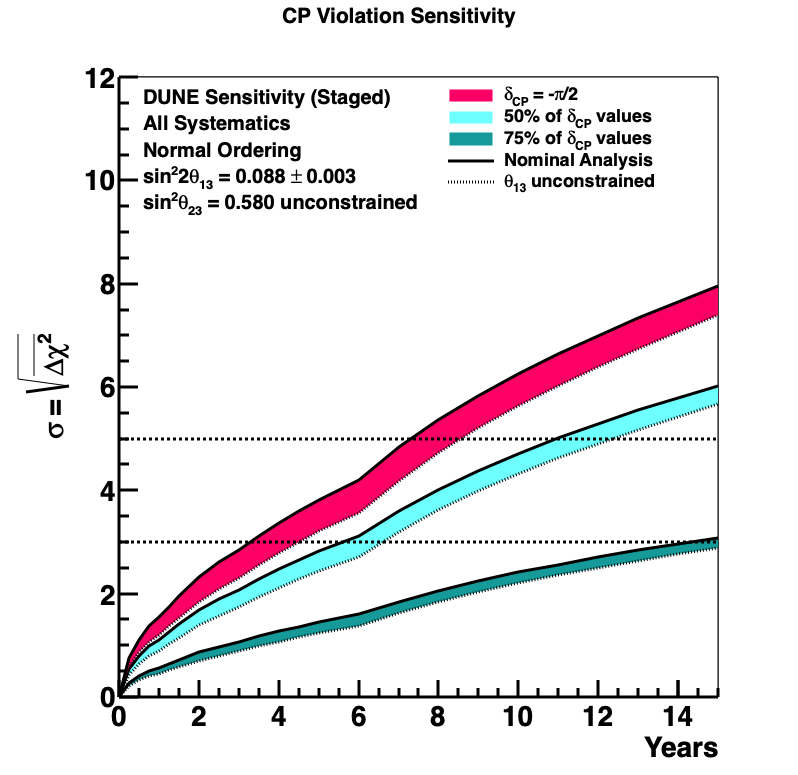
\includegraphics[width=0.95\linewidth]{cpv_exp_staging_varyconstr_nh_2019.png}
\end{dunefigure}

Fig.~\ref{fig:cpv_staging_execsum} 
illustrates DUNE's ability to distinguish 
the value of the \dword{cp} phase \deltacp from \dword{cp}-conserving 
values (0 or $\pi$) as a function of time in calendar year.  
These projections incorporate a sophisticated treatment of systematic 
error, as described in detail in Chapter~\ref{ch:osc}.  
Strong evidence ($>3\sigma$) for \dword{cpv} is obtained for 
favorable values (half of the phase space) of \deltacp after six 
years of running, leading to a $>5\sigma$ determination after 11 years.

A summary of representative sensitivity milestones for neutrino 
mass ordering and \dword{cpv} discovery, as well as precision on 
\deltacp and \sinstt{13} is given in 
Table~\ref{tab:milestones_execsumm}.  The ultimate level of 
precision that can be obtained on oscillation parameters 
highlights the point that DUNE will provide crucial input for  
flavor physics:  Patterns required by particular symmetries 
underlying fermion masses and mixing angles may appear.  The 
unitarity of the neutrino mixing matrix can be tested directly 
through comparisons of \sinstt{13} with the value obtained from 
reactor experiments.  In conjunction with \sinstt{13} and 
other parameters, the precise value of \deltacp may lead to 
constraints on models of leptogenesis that have been proposed 
to explain the baryon asymmetry of the universe.

\begin{dunetable}[Projected DUNE oscillation physics milestones]
{lcc}
{tab:milestones_execsumm}
{Exposure in years, assuming true normal ordering and equal 
running in neutrino and antineutrino mode, required to reach 
selected physics milestones in the nominal analysis, using the 
NuFIT 4.0~\cite{Esteban:2018azc,nufitweb} best-fit values for the oscillation parameters. As 
discussed in Section~\ref{sec:physics-lbnosc-oscvar}, there are 
significant variations in sensitivity with the value of
\sinst{23}, so the exact values quoted here 
(using \sinst{23} = 0.580) are strongly dependent on that choice. 
The staging scenario described in 
Section~\ref{sec:exec-assm-meth-deployment} is assumed. Exposures 
are rounded to the nearest year.}
 Physics Milestone & Exposure (staged years) \\
 5$\sigma$ Mass Ordering & 1 \\
 \phantom{xxx}(\deltacp = -$\pi/2$) & \\ \hline
 5$\sigma$ Mass Ordering & 2 \\
 \phantom{xxx}(100\% of \deltacp values) & \\ \hline
 3$\sigma$ CP Violation & 3 \\
 \phantom{xxx}(\deltacp = -$\pi/2$) & \\ \hline
 3$\sigma$ CP Violation & 6 \\
 \phantom{xxx}(50\% of \deltacp values) & \\ \hline
 5$\sigma$ CP Violation & 7 \\
 \phantom{xxx}(\deltacp = -$\pi/2$) & \\ \hline
 5$\sigma$ CP Violation & 11 \\
 \phantom{xxx}(50\% of \deltacp values) & \\ \hline
 3$\sigma$ CP Violation & 14 \\
 \phantom{xxx}(75\% of \deltacp values) & \\ \hline
 \deltacp Resolution of 10 degrees & 7 \\
 \phantom{xxx}(\deltacp = 0) & \\ \hline
 \deltacp Resolution of 20 degrees & 10 \\
 \phantom{xxx}(\deltacp = -$\pi/2$) & \\ \hline
 \sinstt{13} Resolution of 0.004 & 17 \\ 
\end{dunetable}

%%%%%%%%%%%%%%%%%%%%%%%%%%%%%%%%%%%%%%%%%%%%%%%%%%%%%%%%%%%%%%
\subsection{Proton Decay and Other 
Baryon-number Violating Processes}

By virtue of its deep underground location and large fiducial 
mass, as well as its excellent event imaging, particle 
identification and 
calorimetric capabilities, the DUNE far detector will be 
a powerful instrument for discovery of baryon-number violation.
DUNE will be able to observe signatures of decays of protons and 
neutrons, as well as the phenomenon of neutron-antineutron mixing, 
at rates below the limits placed by the current generation of 
experiments.

Many nucleon decay modes are accessible to DUNE.  
As a benchmark, a particularly compelling discovery channel 
is the decay of a proton to a positive kaon and a neutrino, 
\ptoknubar.  In this channel, the kaon and its decay products 
can be imaged, identified, and tested for kinematic consistency 
with the full decay chain, together with precision sufficient to 
reject backgrounds due to atmospheric muon and neutrino 
interactions. 
Preliminary analysis of single-particle beam and cosmic ray tracks 
in the \dword{pdsp} \lartpc is already demonstrating the particle 
identification capability of DUNE, as illustrated in 
Fig.~\ref{fig:pdsp_dedx_execsum}.  
The signature of the kaon track and its observable decay particles is 
sufficiently rich that a credible claim of evidence for 
proton decay could be made on the basis of just 
one or two sufficiently well-imaged events, for the case 
where background sources are expected to contribute much less 
than one event.
% (see Chapter~\ref{ch:nonaccel} for a more complete 
%discussion). 

\begin{dunefigure}[Reconstructed $dE/dx$ of protons and muons in 
\dshort{pdsp}]{fig:pdsp_dedx_execsum}
{Energy loss of protons (left) and muons (right) in 1-GeV  
running with the \dword{pdsp} \lartpc at CERN, as a function of 
residual range.  The protons are beam particles identified from 
beamline instrumentation; the muons are reconstructed stopping 
cosmic rays collected concurrently.  
The red curves represent the mean of the 
corresponding expected signature.  Note the difference in 
the vertical scale of the two plots.  The kaon $dE/dx$ curve 
will lie between the two curves shown.}
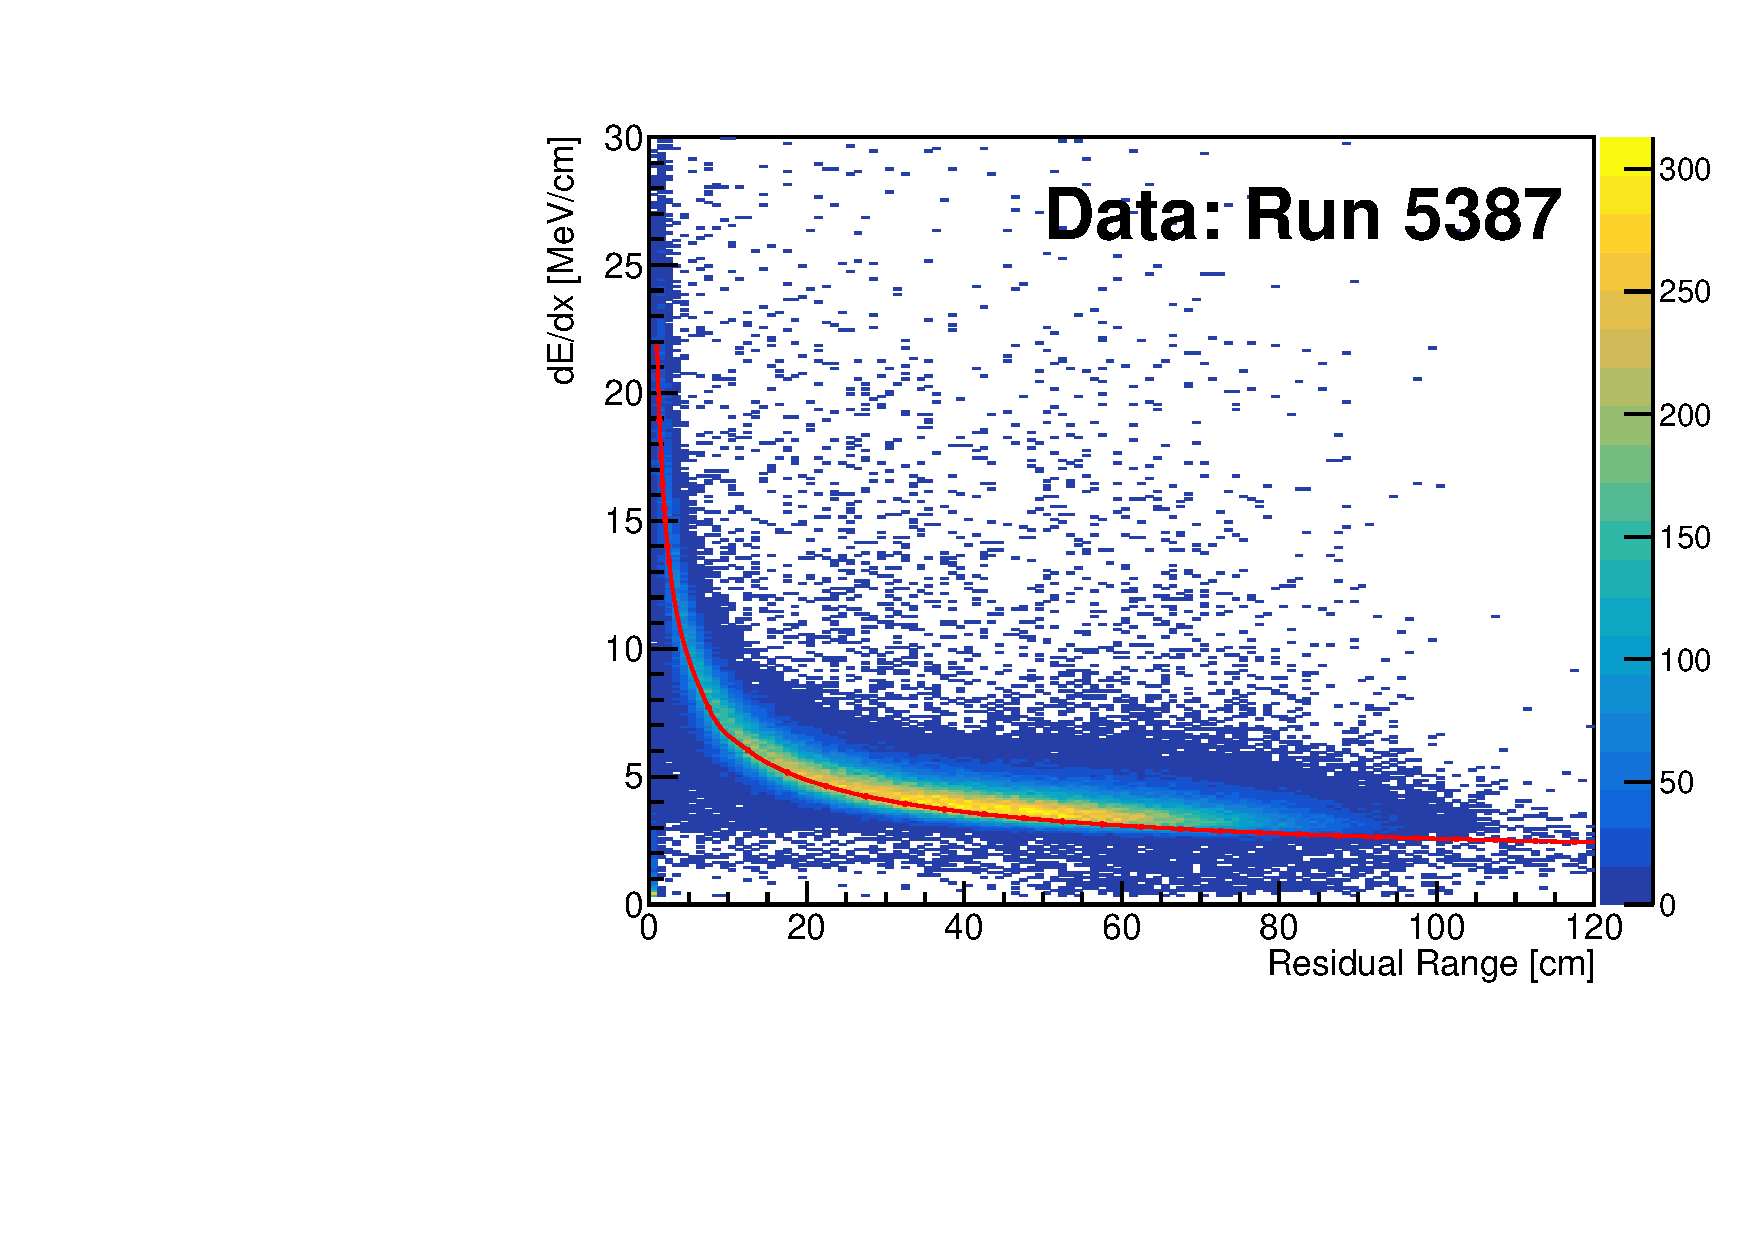
\includegraphics[width=0.45\linewidth]{proton_dedx_resrange_run5387.pdf}\hspace{0.05\linewidth}
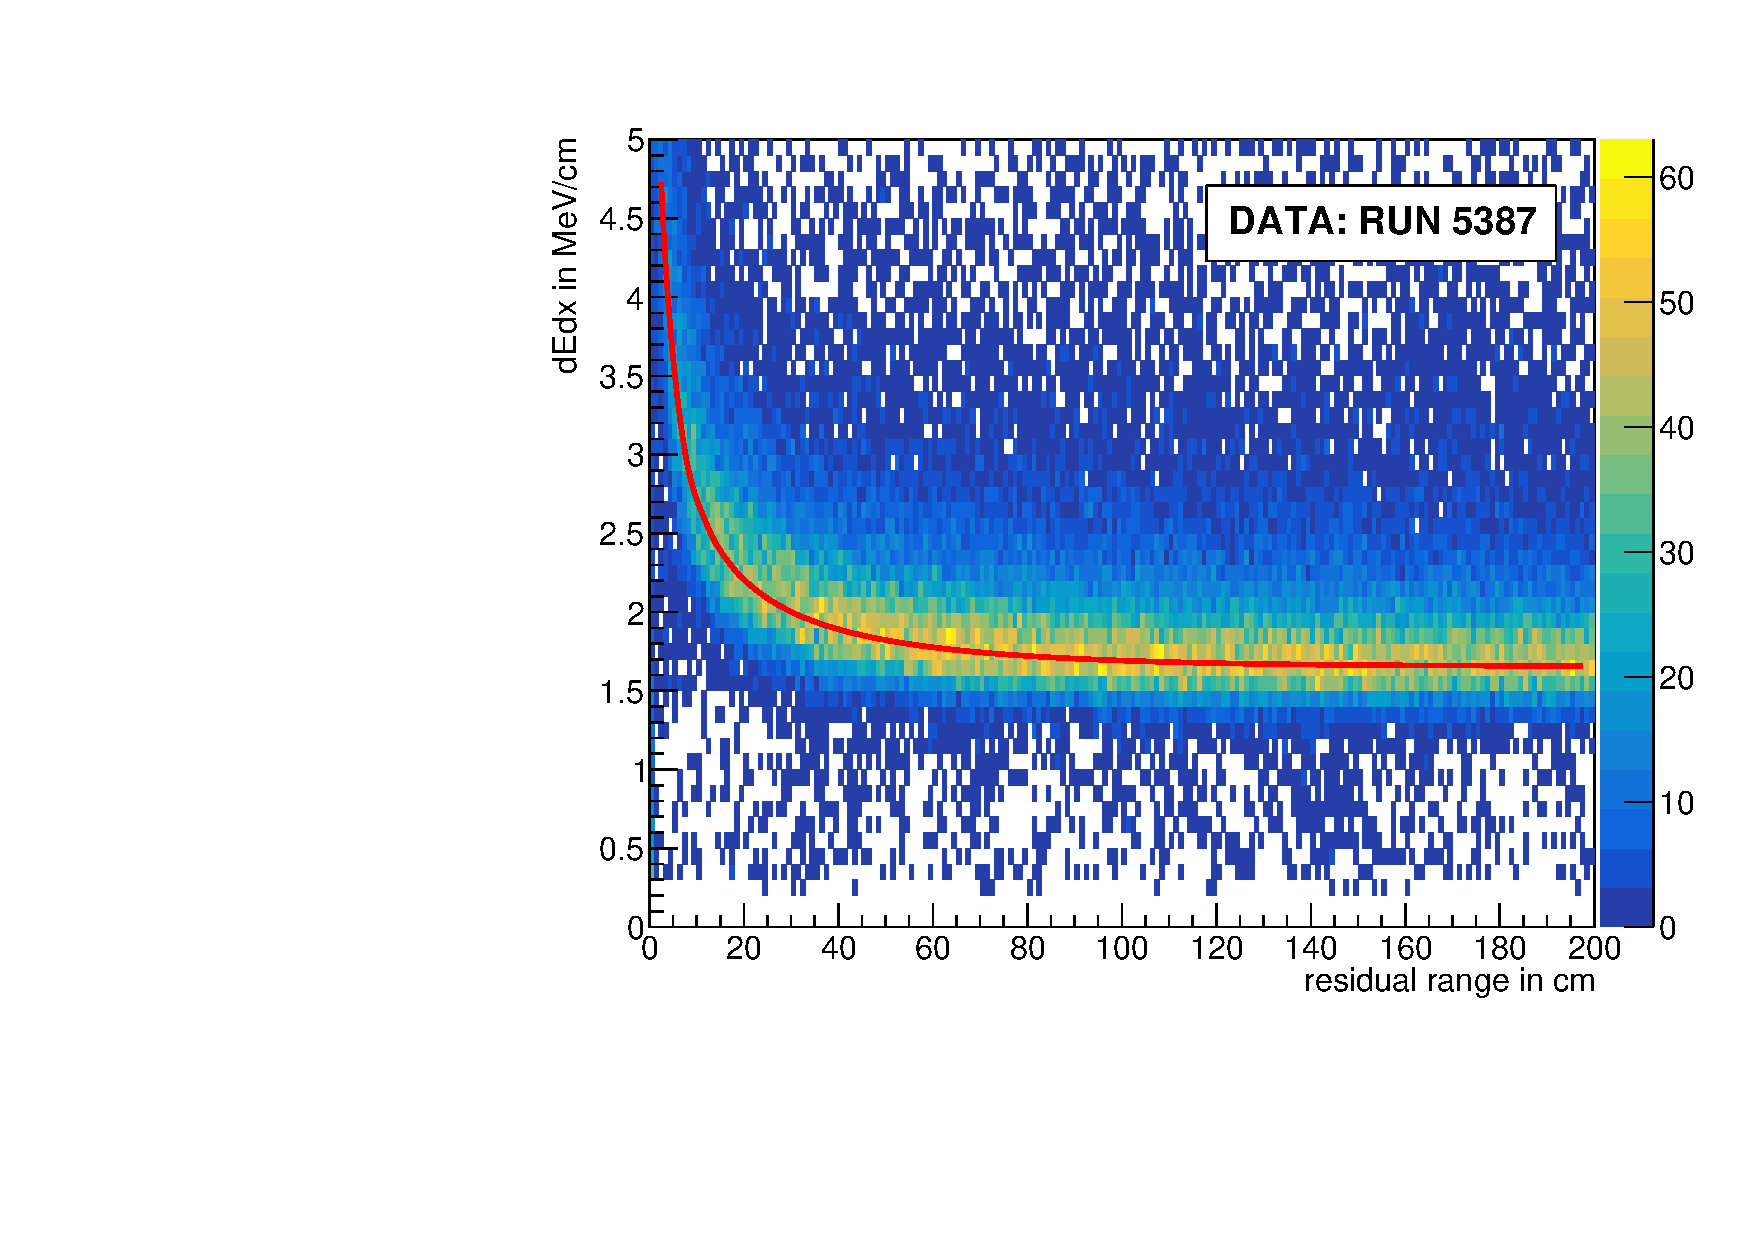
\includegraphics[width=0.45\linewidth]{muon_run5387_dedx.pdf}
\end{dunefigure}

Projecting from the current analysis of \ptoknubar in the DUNE 
far detector, with a detection efficiency of \num{30}\% as 
described in Chapter~\ref{ch:nonaccel}, the 
expected 90\% CL lower limit on lifetime divided by branching 
fraction is \SI{1.3e34}{years} for a 
\num{400}-\SI{}{\ktyr} 
exposure, assuming no candidate events are observed.  This 
is roughly twice the current limit of 
\SI{5.9e33}{years} from \superk~\cite{Abe:2014mwa}, 
based on an exposure of \SI{260}{\ktyr}.  Thus, should the rate 
for this decay be at the current \superk limit, five candidate 
events would be expected in DUNE within ten years 
of running with four far detector modules.  Ongoing work is aimed 
at improving the efficiency in this and other channels.

%%%%%%%%%%%%%%%%%%%%%%%%%%%%%%%%%%%%%%%%%%%%%%%%%%%%%%%%%%%%%%
\subsection{Galactic Supernovae via Measurements of Neutrino Bursts}

As has been demonstrated with SN1987a, the observation 
of neutrinos~\cite{Bionta:1987qt,Hirata:1987hu} from a 
core-collapse supernova can reveal much about these  
phenomena that is not accessible in its  
electromagnetic signature.  Correspondingly, there is a 
wide range of predictions from supernova models for even 
very basic characteristics of the neutrino bursts.  Typical  
models predict that a supernova explosion in the 
center of the Milky Way will result in several thousand 
detectable neutrino interactions in the DUNE far detector 
occurring over an interval of up to a few tens of seconds.
The neutrino energy spectrum peaks around \SI{10}{MeV}, 
with appreciable flux up to about \SI{30}{MeV}.

\lar based detectors are sensitive to the \nue 
component of the flux, while water Cherenkov and organic 
scintillator detectors are most sensitive to the \anue 
component.  Thus DUNE is uniquely well-positioned to study the 
neutronization burst, in which \nue's are produced during the 
first few tens of milliseconds.  More generally,  
measurements of the (flavor-dependent) neutrino flux and energy 
spectrum as a function of time over the entirety of the burst 
can be sensitive to astrophysical properties of the supernova 
and its progenitor, and distortions relative to nominal 
expectations can serve as signatures for phenomena such 
as shock wave and turbulence effects, or even black hole 
formation.  

An illustration 
of one element of the program is given in Fig.~\ref{fig:fullSN_execsum}, 
which indicates a pointing resolution of better than $5^\circ$ that 
can be obtained by analysis of both subdominant highly-directional $\nu$-$e$ elastic scattering 
events and dominant weakly-directional $\nu_e$CC events within a supernova burst, based 
on full reconstruction and analysis. The DUNE results can be 
combined with corresponding measurements in other neutrino detectors to 
provide supernova localization from neutrinos alone in real time.
%
\begin{dunefigure}[Supernova direction determination from $\nu-e$ elastic scattering events]{fig:fullSN_execsum}{Left: Log
    likelihood values as a function of direction for a
    supernova sample with 260 $\nu$-$e$ elastic scattering (ES) events.  Right: Distribution of angular differences for
    directions to 10-kpc supernova using a maximum likelihood
    method.}
  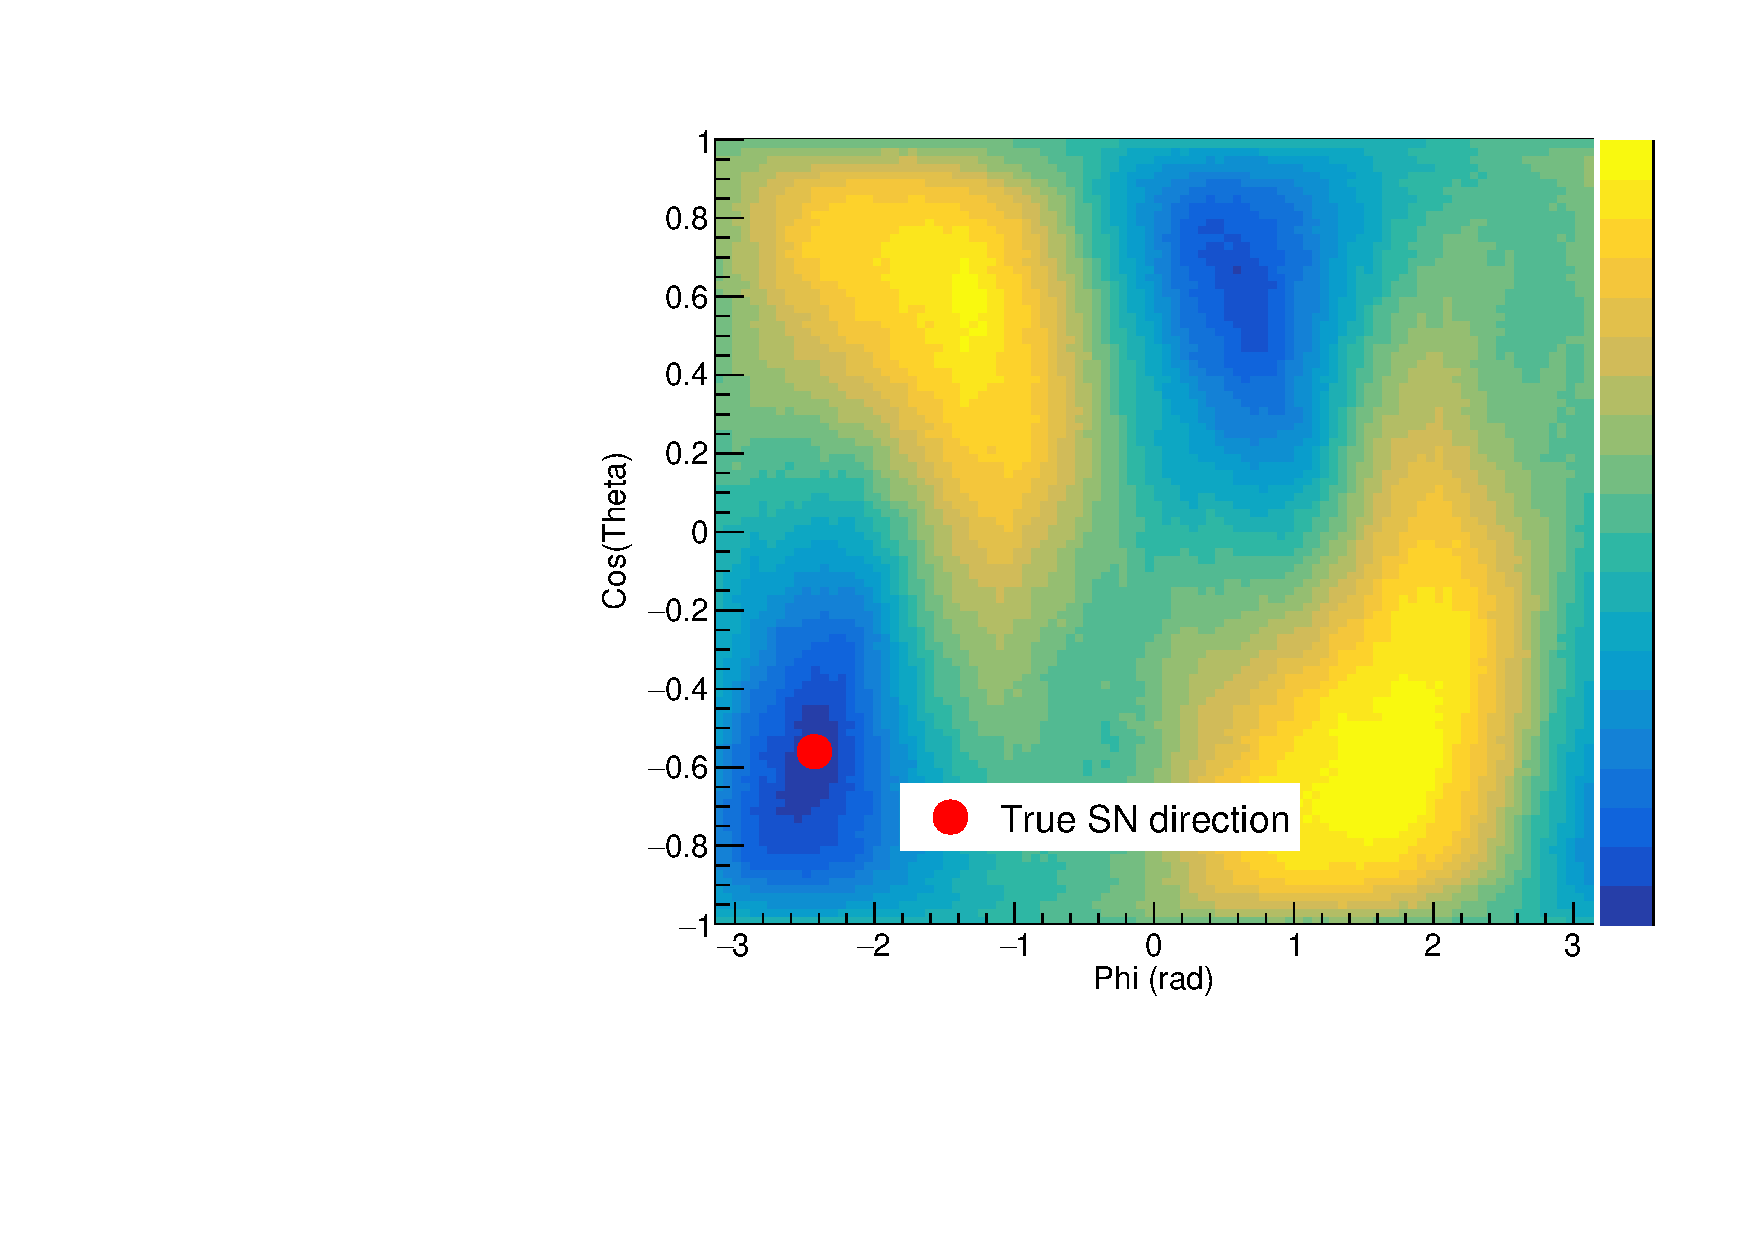
\includegraphics[width=0.44\textwidth]{LLH_252_SNdir.pdf}
  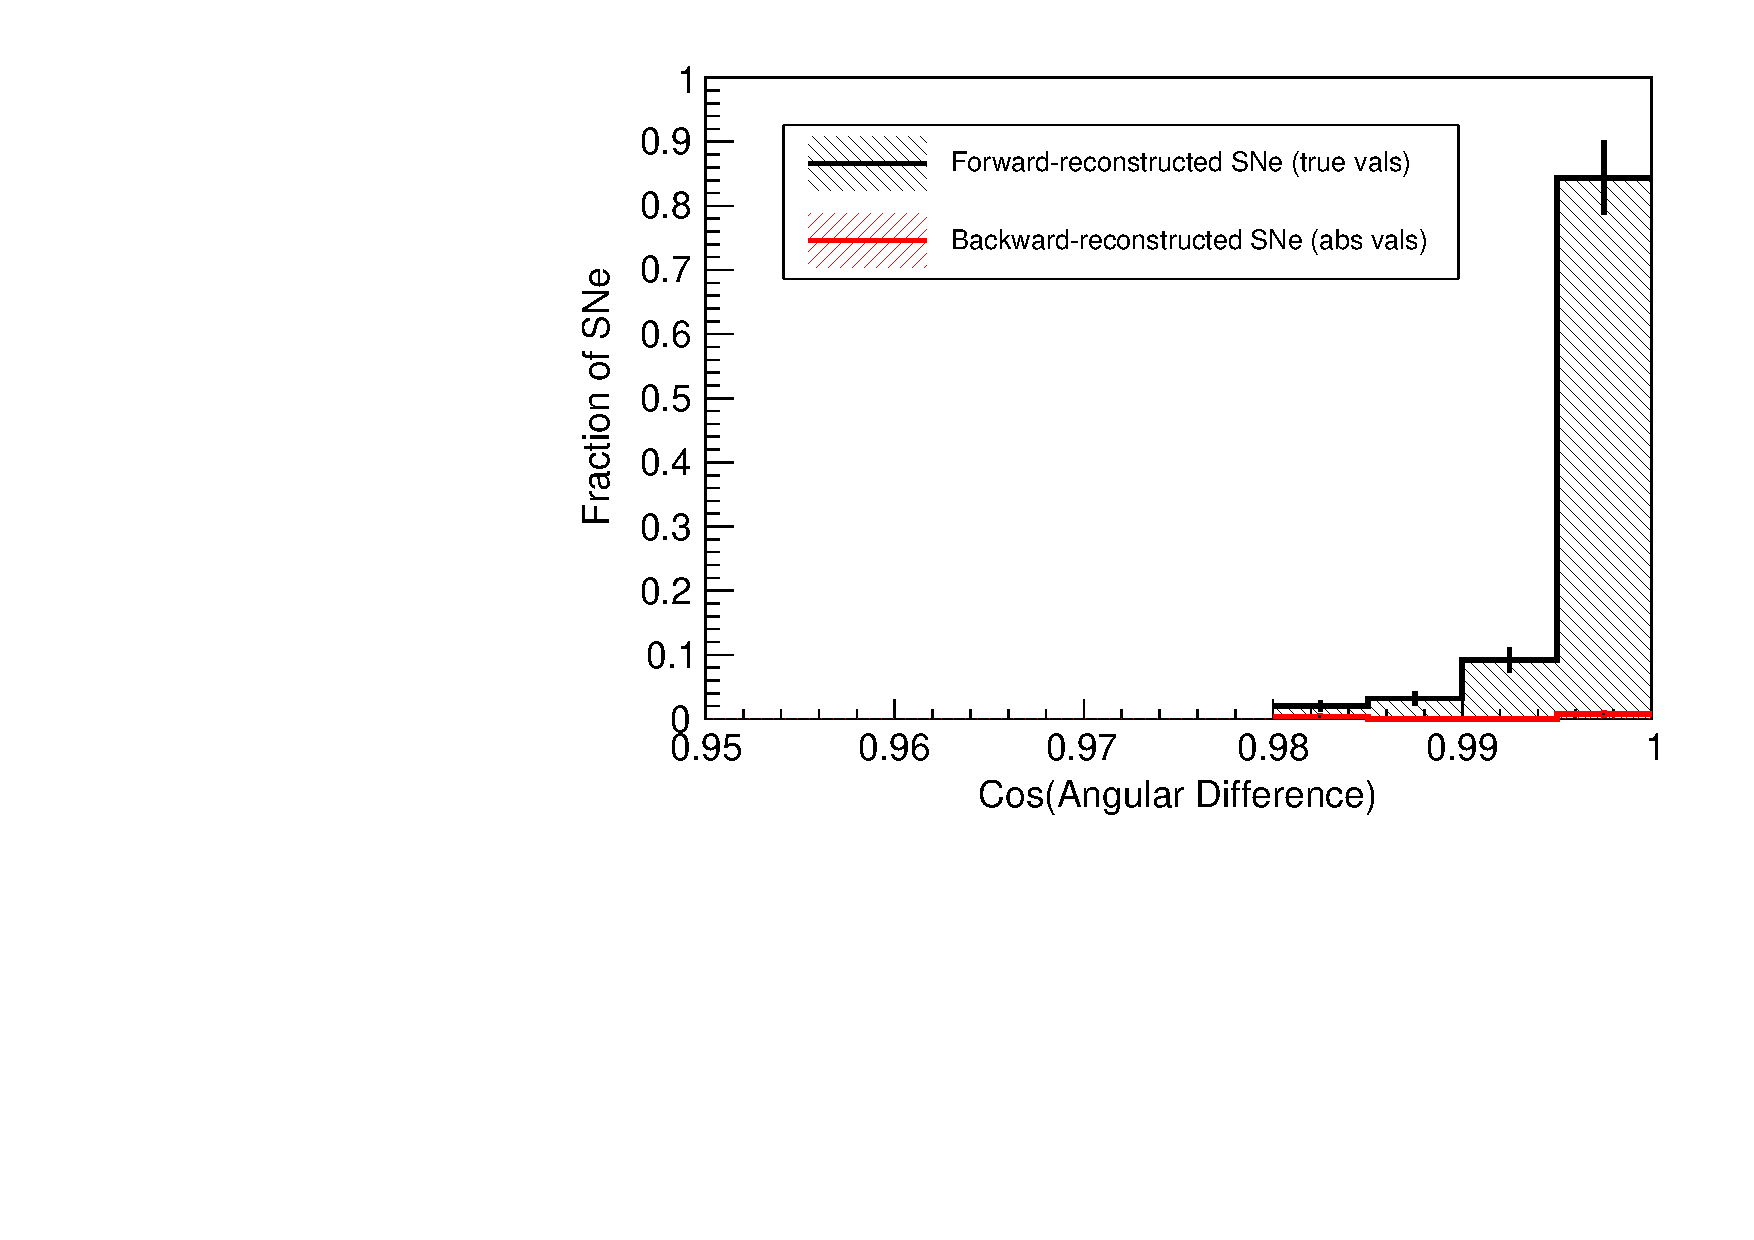
\includegraphics[width=0.48\textwidth]{costheta_fullSN_ESCCPDFs_TDR.pdf}
\end{dunefigure}

%%%%%%%%%%%%%%%%%%%%%%%%%%%%%%%%%%%%%%%%%%%%%%%%%%%%%%%%%%%%%%                                   
\section{Science Drivers for LBNF/DUNE Design Specifications}
\label{sec:exec-phys-key-reqs}

The scientific case summarized in the sections above
is predicated on the suitability of the experimental
configuration of LBNF/DUNE.  In this section we summarize
the ways in which the primary physics goals drive key features
of this configuration.  
Translation of performance needs into the
corresponding LBNF/DUNE design specifications is addressed within
the appropriate TDR volume.

%\subsection{Far detector performance requirements}
%\label{sec:exec-phys-fd-requirements}

The number of detector design parameters that have direct
or indirect impact on performance is large.  These design
parameters have been studied over the years by past LArTPC
experiments, by DUNE during early detector optimization work,
through the successful construction and now operation of
ProtoDUNE-SP, and through continuing studies within the
DUNE consortia and physics groups.

\subsection{High-level Observables in the Far Detector}

DUNE's suite of physics measurements relies on a relatively small
number of event observables, through which the physics of interest
can be accessed.  Foremost are:
%                                                                                                
\begin{itemize}
\item {\bf Particle energies}  \\
Examples include the total visible energy in a supernova
neutrino interaction; the reconstructed energy of a beam
neutrino for oscillation measurements; the reconstructed
energy of a muon track in a nucleon decay candidate event.

\item {\bf Particle identification}  \\
This comes from spatial patterns and energy depositions.
Examples include photon/electron separation in the \nue{}
appearance analysis; proton/kaon separation in certain
nucleon decay channels.

\item {\bf Event time} \\
This allows for fiducialization
in the TPC, drift corrections, and macroscopic timing for
beam neutrinos and supernova neutrino bursts.
\end{itemize}



\subsection{Physics Case Studies}

\paragraph{\bf CP violation search}
The primary demonstration that the detector design meets
the physics needs is the full simulation and analysis
being documented in this TDR volume.  As described in 
Sec.~\ref{sec:exec-sensitiv-results}, 
Figure~\ref{fig:cpv_staging_execsum}
presents the time-evolution of the \dword{cpv} sensitivity 
obtained in this way.


To break the measurement apart into the three
observables above, we start with neutrino energy.
The charged lepton and hadronic shower energies are
reconstructed separately and then summed.  In electron
neutrino events, the leptonic energy resolution
(spectrum averaged) is 8\%, the hadronic energy resolution
is 49\%, and the neutrino energy resolution is 13\%.
Note that a significant portion of the energy smearing
comes from the physics of neutrino-nucleus scattering
and hadronic shower production rather than from detector
performance.  In the impossible case that the lepton
energy could be perfectly reconstructed, the electron
neutrino (muon neutrino) energy resolution would only
change by approximately $13\%\rightarrow 10\%$ 
($18\%\rightarrow 17\%$).
Equivalently, small degradations in detector response
have minimal leverage to affect the final neutrino energy
resolution.

Particle identification is critical for the oscillation analysis 
in that it enables neutrino flavor identification.  
For \nue{} appearance in particular, one
must positively identify the presence of a high-energy
electron while avoiding misclassification of high energy
photons as electrons. The LArTPC design meets this challenge
by having spatial resolution that is much smaller than the
radiation length ($0.5~\rm{cm} \ll 14~\rm{cm}$) to make
visible the gaps between an event's reconstructed vertex
and any photon conversions, and charge resolution that
provides additional $dE/dx$ separation based on pre-EM-shower
depositions, as demonstrated in an operating detector by
ArgoNeuT~\cite{Acciarri:2016sli} and with DUNE simulation
in Figure~\ref{fig:emdedx}.  The DUNE study~\cite{bib:docdb3384}
also shows alternative detector designs for the 
single-phase \lartpc implementation.  As long as
the signal-to-noise ratio is high on the readout wires,
minor adjustments to the wire angle and pitch have negligible
impact on $dE/dx$ separation power.
%
\begin{dunefigure}
[Separation of photons and electrons by $dE/dx$
in the pre-shower region]
{fig:emdedx}
{Separation of photons and electrons by $dE/dx$
in the pre-shower region.  Alternative wire angles and wire
pitches are also shown.}
  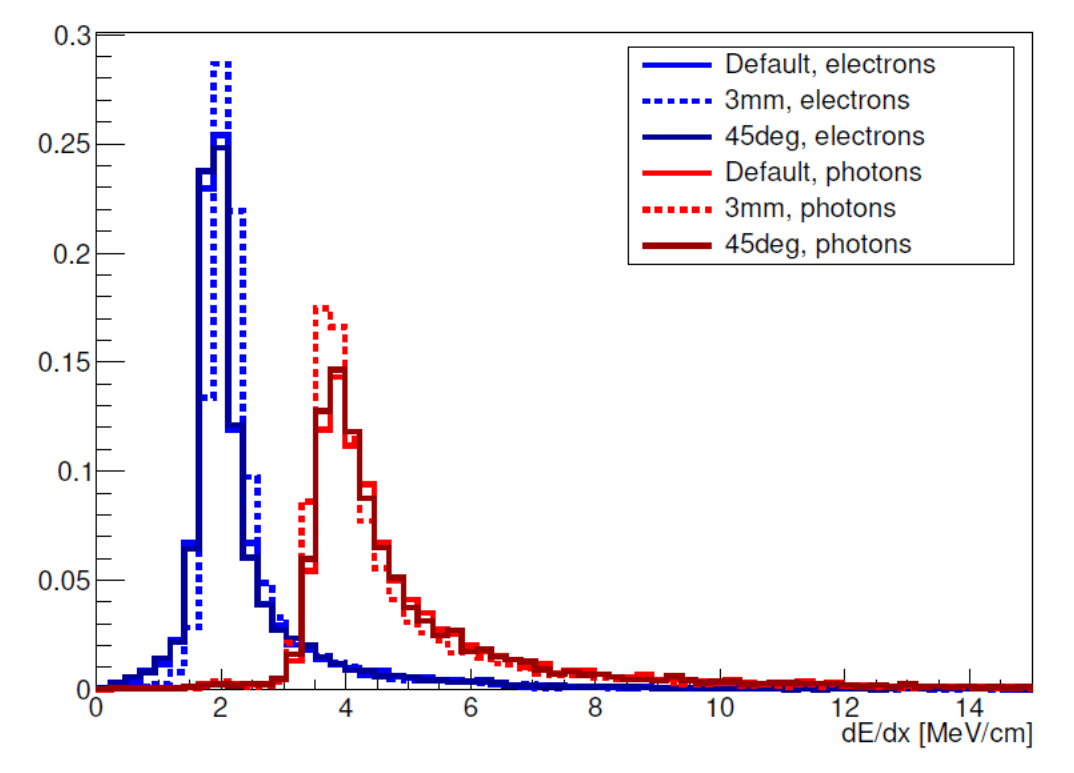
\includegraphics[width=0.7\linewidth]{emdedx.png}
\end{dunefigure}

In the analysis presented in Chapter~\ref{ch:osc}, and in
the preliminary \dword{cpv} sensitivity in
Figure~\ref{fig:cpv_staging_execsum}, neutrino flavor classification
is accomplished using a modern convolutional neural network
technique that takes directly as input the TPC wire hits
in the three detector views.

Event timing requirements for beam events flow from the
need to establish the fiducial volume.  This is discussed
generally in the section on light yield below.

\noindent {\bf Supernova burst neutrinos.}  A core-collapse
supernova at 10~kiloparsecs will provide $\sim$1000 neutrino
interactions in the Far Detector over the course of
$\sim$10 seconds with typical energies between 5 and 30~MeV.
Charged current \nue{} events make up the majority of these.
Much of the desired astrophysical information comes via the
time-dependent energy spectrum of these neutrinos.  As shown
earlier in Sec.~\ref{sec:exec-sensitiv-results} and later
in more detail in Chapter~\ref{ch:snb-lowe},
DUNE capabilities are quantified through sensitivities
both to generic pinched-thermal spectral parameters 
and to
specific phenomena within the star.

Figure~\ref{fig:specpars} shows the precision with which DUNE
can measure two of the spectral parameters, $\varepsilon$, related to
the binding energy of the neutron star remnant, and $\langle
E_{\nu_e}\rangle$, the average energy of the $\nu_e$ component, for the
time-integrated spectrum.
The assumed measured spectrum takes into account some degradation
from the neutrino interaction process itself 
({\em e.g.}, energy lost to neutrons), via the ``MARLEY'' model.
The colored contours show increasing levels of energy smearing.
A 10\% resolution is noticeable but insignificant, and the
overall precision on the spectral parameters up to 30\%
resolution does not change dramatically.
The additional smearing introduced by the detector's response
falls within the resolution envelope suggested here, and according to
detector simulation is closest to the 20\% level.
In an eventual detailed analysis, the spectral
fits will be done in time slices to study the evolution of
the supernova, so the minimum contour size in each time slice
will be larger due to reduced event counts in each slice.

\begin{dunefigure}
[90\%~C.L.\ contours for spectral parameters for a supernova
at 4~kpc.]
{fig:specpars}
{90\%~C.L.\ contours for the luminosity and average $\nu_e$ energy
spectral parameters for a supernova
at 4~kpc.  The contours are obtained using the time-integrated
spectrum.  As discussed in the text, the allowed regions
change noticeably but not drastically as one moves from
no detector smearing (black) to various realistic resolutions (colors).
The jagged shapes in this preliminary plot are due to binning.}
  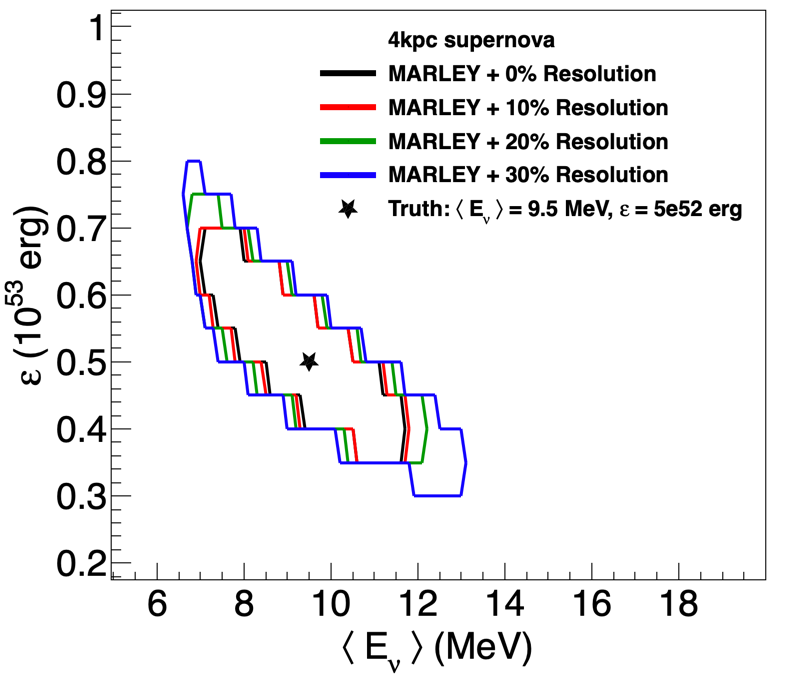
\includegraphics[width=0.7\linewidth]{EnergyResolution_4kpc_TDR.png}
\end{dunefigure}

Given the dominance of \nue{} charged current events in the
supernova neutrino sample, particle identification is not a
requirement for the primary physics measurements.  However,
additional capability may be possible by identifying separately
neutral current and elastic scattering interactions.  


Timing for supernova neutrino events is provided by both the
TPC and the photon detector system.  Basic timing requirements
flow from event vertexing and fiducialization needs.  These are
discussed generally for DUNE in the light yield section, but
here we note a few supernova-specific design considerations.
During the first 50~ms of a 10-kpc-distant supernova, the
mean interval between successive neutrino interactions is
$0.5 - 1.7~\rm{ms}$ depending on the model.  The TPC alone
provides a time resolution of 0.6~ms (at 500~V/cm), commensurate
with the fundamental statistical limitations at this distance.
However nearly half of galactic supernova candidates lie closer
to Earth than this, so the rate can be tens or (less likely)
hundreds of times higher.  A resolution of $\mathord{<}10~\mu\rm{s}$,
as already provided by the photon detector system, ensures that
DUNE's measurement of the neutrino burst time profile is always
limited by rate and not detector resolution.  The hypothesized
oscillations of the neutrino flux due to standing accretion shock
instabilities would lead to features with a characteristic time
of $\sim$10~ms, comfortably greater than the time resolution.
The possible neutrino trapping notch at the start of the burst
has a width of $1 - 2~\rm{ms}$.  Observing the trapping notch
could be possible for the closest progenitors.

\subsection{Key High-level Detector Design Specifications}

With the discussion above and in later chapters of this 
document, it is possible to identify several high-level 
detector design parameters that together characterize the  
overall function of DUNE single-phase \lartpc modules.  These 
parameters and specified operating points are given in 
Table~\ref{tab:exec-fd-specs}.
%
\begin{dunetable}[High-level DUNE single-phase far detector design specifications]
{lll}
{tab:exec-fd-specs}
{High-level DUNE single-phase far detector design parameters 
and specifications}
Parameter & Specification & Goal\\ \toprowrule
Drift field       & $>\SI{250}{\volt/\cm}$     & 500~V/cm\\
Electron lifetime & $>\SI{3}{\milli\second}$   & 10~ms\\
System noise      & $<1000$~enc & --- \\
Light yield (at cathode)  & $>\SI{0.5}{pe/\MeV}$ & $>\SI{5}{pe/\MeV}$\\
%Photon detection threshold       & $>\SI{5}{\MeV}$ &  $>\SI{0.5}{\MeV}$\\
%Light yield       & $>\SI{0.5}{pe/\MeV}$ & $>\SI{13}{pe/\MeV}$\\
Time resolution   & $<\SI{1}{\micro\second}$    & 100~ns\\
\end{dunetable}
%

The column headings in the table are defined as follows:
\paragraph{Specification:} This is the intended value for the parameter or, more often, the 
upper or lower limit for the parameter.  Fixed values are given for parameters that are not intrinsically dynamic ({\em e.g.}, wire pitch).  Limits are set by the more stringent driver, either
 the physics or engineering needs.

\paragraph{Goal:} This is an improved value that offers some benefit, and the collaboration
aims to achieve this value where it is cost effective to do so.  While in some cases the goal offers potential physics benefit directly, more often the goal provides risk mitigation, since improving the performance on one parameter can mean relaxing the requirements on other correlated parameters, thus protecting against unforeseen performance issues.

The first three parameters (drift field, electron lifetime, 
and TPC system noise) in Table~\ref{tab:exec-fd-specs} 
enter directly into the ability to discriminate between 
ionization signals due to physics events and noise.  Physics 
capability degrades if readout noise is not small compared to 
the ionization signal expected for minimum-ionizing particles
located anywhere within the active volume of the detector.
The remaining parameters (light yield for events at the cathode, 
and timing resolution) pertain to the ability 
of the scintillation photon detection system to enable 
localization of events within the TPC, needed for the 
non-accelerator based far detector physics program, both 
for fiducialization and for corrections to TPC charge 
attenuation.  The general 
arguments for the specifications listed for each parameter 
are given below.

\paragraph{Drift field}
The basic operating principle of the TPC involves the transport 
of ionization electrons out of the argon volume and to the 
detection plane.   
A higher drift field reduces electron transport time 
and thus electron loss due to impurities; 
reduces ion-electron recombination (increasing ionization signal at the expense of reduced scintillation photon yield); increases induction 
signals due to increased electron velocity; and reduces 
electron diffusion.


The argon volume in the Far Detector single phase design is 
divided into four separate drift regions, each with a maximum 
drift distance of 3.5~m.  The design goal of 500~V/cm field 
implies a voltage across the drift region of approximately 
180~kV.  At this field, the electron drift velocity is 
1.6~mm/$\mu$s , implying a maximum drift time $t=2.2~\rm{ms}$.  
This drift time can be compared with the electron lifetime 
$\tau$ set by the argon purity.  At $\tau=3~\rm{ms}$, signals
originating near the cathode will be attenuated to 
$e^{-t/\tau} = 48\%$ of their original strength.  
For the minimum field of 250~V/cm, this transmission becomes 
23\%.  Additionally, electron/ion recombination happens more 
readily at lower field.  From 500~V/cm to 250~V/cm, 
an additional signal loss of 11\% (taking 23\% to 20\%) is 
introduced due to recombination.  The lowered field also 
reduces the drift velocity and, in proportion, signal pick-up 
on the induction wires.  Moving from 500~V/cm to 250~V/cm drops 
the induction signal by an additional 34\% to an effective
transmission for low-field depositions near the cathode 
(relative to ``500~V/cm near the anode'') of 14\%.

These signal attenuations are acceptable as long as the readout 
maintains good \dword{s/n} ratio and charge resolution.  High \dword{s/n} for 
\dword{mip} signals has been demonstrated at ProtoDUNE-SP --  \dword{s/n}=30 
(collection), 15 (induction) -- and the minimum transmissions 
above would not significantly damage the ability to identify 
wire hits.  The charge resolution on individual wires, while not 
a driver of overall event resolution, feeds into $dE/dx$ 
estimation for short segments of tracks and thus into 
particle identification.  Studies of selection efficiencies at 
varied signal levels continue, but notably the \nue 
selection efficiency exhibits no dependence on drift 
difference in the default simulation, which is based on a 
3~ms electron lifetime.  As mentioned below, ProtoDUNE readily 
achieved higher lifetimes.

Electrons drifting across the full 3.5~m will experience 
transverse diffusion of 1.7~mm (2.0~mm) at 500~V/cm (250~V/cm).  
The change in diffusion with field strength is insignificant in comparison to the wire pitch of 5~mm.

The reduced recombination at higher field results in 
smaller scintillation photon yields.  At 500 V/cm, the 
yield is 60\% of that at zero field.  Thus any reduction 
in field strength will improve this detection channel.  
However, the incremental nature of this improvement and 
the more critical dependence of successful execution of 
the science program on the TPC performance together make
optimization with respect to scintillation a secondary consideration.

ProtoDUNE-SP is currently operating at 500~V/cm.

\paragraph{Electron lifetime}
Electronegative impurities ({\em e.g.}, $\rm{H}_{2}\rm{O}$, $\rm{O}_{2}$) within the liquid argon must be kept at 
low levels to prevent the capture of drifting electrons after ionization.  Electron lifetime is inversely proportional to the level of these impurities.

The values in Table~\ref{tab:exec-fd-specs} correspond to 
contamination levels of of 100 ppt $\rm{O}_2$-equivalent 
for 3~ms and 30~ppt for 10~ms.  The influence of electron 
lifetime on physics capabilities has been discussed in the 
section on drift field above.  
Indeed, one can largely trade off purity for field. 
Note that the lower lifetime of 3~ms was assumed throughout 
that section, versus the goal of 10~ms.  ProtoDUNE-SP has achieved electron lifetimes exceeding 5~ms.

\paragraph{Electronics system noise}
Noise in the electronics system can 
limit the ability to identify and correctly associate wire hits 
and can worsen charge resolution.  From engineering
considerations, the noise level in the front-end electronics 
drives the specification.  All other pieces of the electronics 
chain are to be kept well below this level.  
The specification is given in units of $e^-$ equivalent 
noise charge (enc).

At current gain settings, 1000~enc corresponds 
to 6.5 ADC counts.  Initial ProtoDUNE analyses are 
showing 3.5 (4.5) ADC counts on collection (induction) channels. 
The current \dword{fd} simulation assumes a noise level similar to 
ProtoDUNE performance, but higher noise levels are being 
explored.  It is not expected that these relatively small
adjustments (factor of $\sim$2) will impact physics analysis 
in any significant way.  Noise assumptions (level and 
correlations) do influence DAQ design choices.

\paragraph{Light yield and photon-based timing}
The photon detector system provides an event time 
based on the scintillation light produced in the liquid argon.  
In conjunction with the TPC ionization signal, this allows 
one to determine where the event occurred along 
the drift direction for event vertexing, fiducialization, 
and electron attenuation corrections.  The 
specifications here are given for the worst-case event 
location in the fiducial volume, typically near the cathode 
and thus far from any photon detector on the anode planes.

A photon-based time resolution of 1~$\mu$s corresponds to the 
time resolution for single TPC wire hits, allowing for useful 
event matching between the TPC and photon detector systems.  
Given the drift velocity, 1~$\mu$s also corresponds to an 
effective spatial granularity in the drift direction 
($\sim$2~mm) that is similar to the wire pitch.  The resulting 
three-dimensional event vertex provided by combining TPC and 
photon detector information has essential uses in DUNE physics 
analyses.  A fiducial volume must be defined at the 
$\mathord{<}1\%$ level for the accelerator-based neutrino 
oscillation measurements and for nearby supernovas, and at less 
stringent levels for other measurements.  Additionally, most 
cosmogenic and environmental backgrounds for non-accelerator 
measurements ({\em e.g.}, neutral particles produced by cosmic 
rays in the surrounding rock) have tell-tale distributions in the
active volume and can thus be mitigated or eliminated through 
event localization.

The precise event time, and thus event location, also allows a 
correction for electron attenuation, which otherwise could have 
a large effect on energy resolutions due to the non-uniformity
of response across the drift volume.  
The minimum TPC performance 
considered (with $E=250~\rm{V/cm}$, $\tau=3~\rm{ms}$) would 
correspond to an energy smearing of 22\% due to electron loss.  
This effect is made negligible at 1~$\mu$s time resolution.

This attenuation correction is only possible when photon signals can be successfully associated with a TPC-recorded event.  For low energy supernova neutrino events, this association is not 
100\% efficient.  Figure~\ref{fig:tpcres} shows the smearing on visible energy in the TPC for supernova neutrino events with and without a drift correction based on different photon detector system performance.  The difference between no correction and any correction is dramatic.  The small differences between different light levels (cast as effective photodetector area in the figure) stem not from improved spatial resolution but from a higher efficiency at reconstructing and associating light signals with the TPC signals.  An effective area of 23~$\rm{cm}^2$ corresponds roughly to a light yield of 0.5~p.e./MeV at the cathode, {\em i.e.}\ the minimum specification.
%
\begin{dunefigure}
[Dependence of reconstructed \dshort{snb} event energy on timing-based drift correction]
{fig:tpcres}
{Energy residuals for supernova neutrino events without (black) 
and with (color) a timing-based drift correction to the 
reconstructed energy.  The red histogram assumes the event 
vertex is known perfectly, and the realistic cases approach that
ideal quickly.  The $23~\rm{cm}^2$ histogram roughly corresponds 
to the specification of 0.5~p.e./MeV.}
  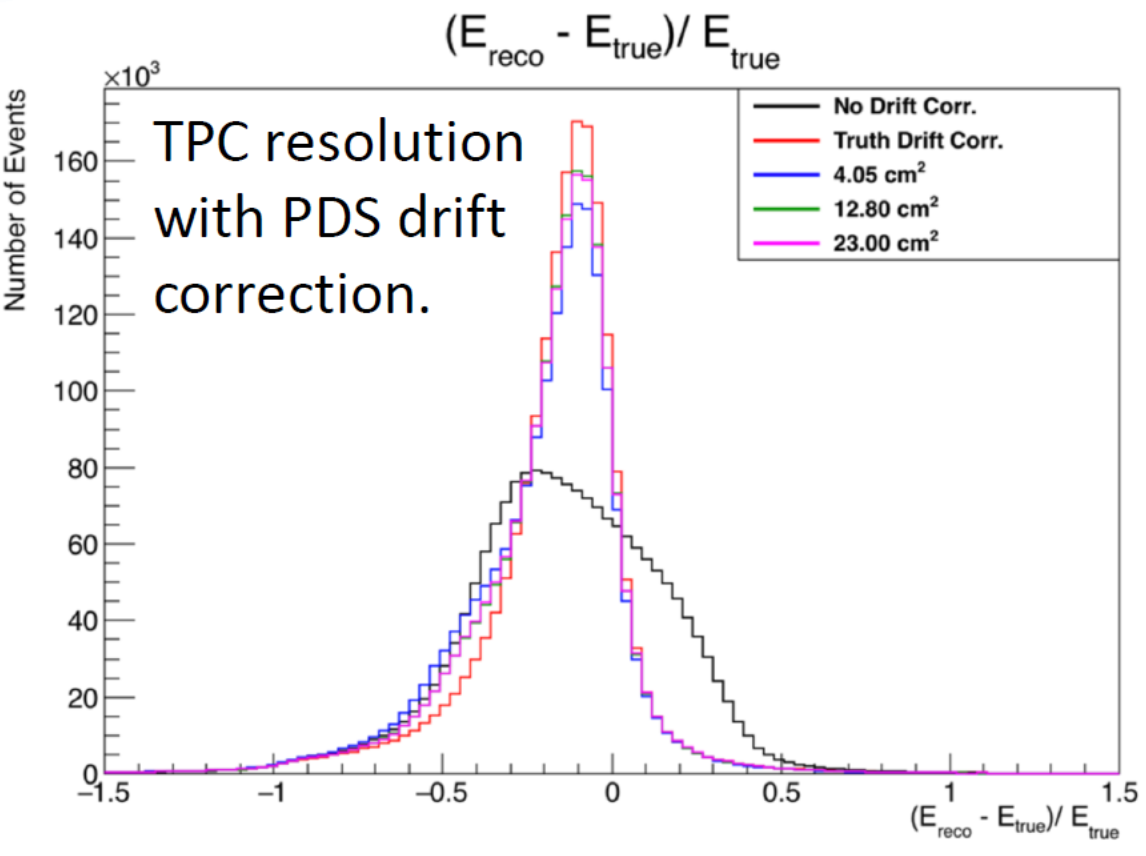
\includegraphics[width=0.7\linewidth]{tpcres.png}
\end{dunefigure}

The use of photon signals for direct event calorimetry in 
supernova neutrino events is under study. Initial tests suggest 
resolutions around 25\% are possible at 0.5 p.e./MeV, which is
competitive with the TPC resolution at these energies.

Two light-collection bar designs and one segmented design 
(ARAPUCA) are operating in ProtoDUNE-SP.  Initial performance 
evaluation is excellent, and a full quantitative assessment, 
described in Volume~\volnumbersp{}, \voltitlesp{}  
is in progress.

\subsection{Detector Design Driver Summary}

The above discussion provides the basic guidelines for key far 
detector performance specifications in the context of the 
single-phase module design.  Further elaboration is given in the 
chapters devoted to science capabilities in 
Volume~\volnumberphysics{}, \voltitlephysics{}.
Discussion of other significant detector specifications 
and their impact on 
physics sensitivity is given in Volumes~\volnumbersp{} and~\volnumberdp{}, \voltitledp{}.  While it is not practical to carry out 
comprehensive physics sensitivity studies comprehensively, in 
which every major detector parameter is varied individually or 
in conjunction with others, such studies have been done 
for a few significant parameters (such as anode wire pitch for 
the single-phase \lartpc design).  These are reported in the 
corresponding detector volume.


%%%%%%%%%%%%%%%%%%%%%%%%%%%%%%%%%%%%%%%%%%%%%%%%%%%%%%%%%%%%%%
%%%%%%%%%%%%%%%%%%%%%%%%%%%%%%%%%%%%%%%%%%%%%%%%%%%%%%%%%%%%%%

